\section{UI Sketches}
\setlength{\parindent}{0ex}
\subsection{Simulator}

Die Navigation im Simulator ist in vier Schritte eingeteilt:
\begin{itemize}
    \item Auswählen von zu simulierenden Stationen
    \item Erstellen von Generierungspresets
    \item Zuweisen dieser Presets zu den einzelnen Stationen
    \item Simulieren der Messdatengenerierung mit Live-Visualisierung
\end{itemize}

Die einzelnen Stages werden mithilfe eines Tab-Controlls umgesetzt und man kann jederzeit, wenn die Simulation gestoppt ist, Einstellungen vornehmen.

\subsubsection{Stationen auswählen}

Alle verfügbaren Stationen werden in der rechten Liste (siehe Abbildung \ref{fig:sketch_select_station}) angezeigt. 
Beide Listen verfügen über eine Filterungsmöglichkeit (TextBox), die sich oberhalb der jeweiligen Liste befindet.
Die Pfeile zwischen den Spalten dienen nur zu visuellen Betonung, dass die Stationen per Mausklick von der einen Spalte in die andere verschoben werden können. Nachdem alle zu simulierenden Stationen ausgewählt wurden, kann man entweder durch Klicken des \grqq Weiter\glqq-Buttons oder durch Auswählen des nächsten Tabs zum nächsten Schritt gewechselt werden.

\begin{figure}[H]
\centering
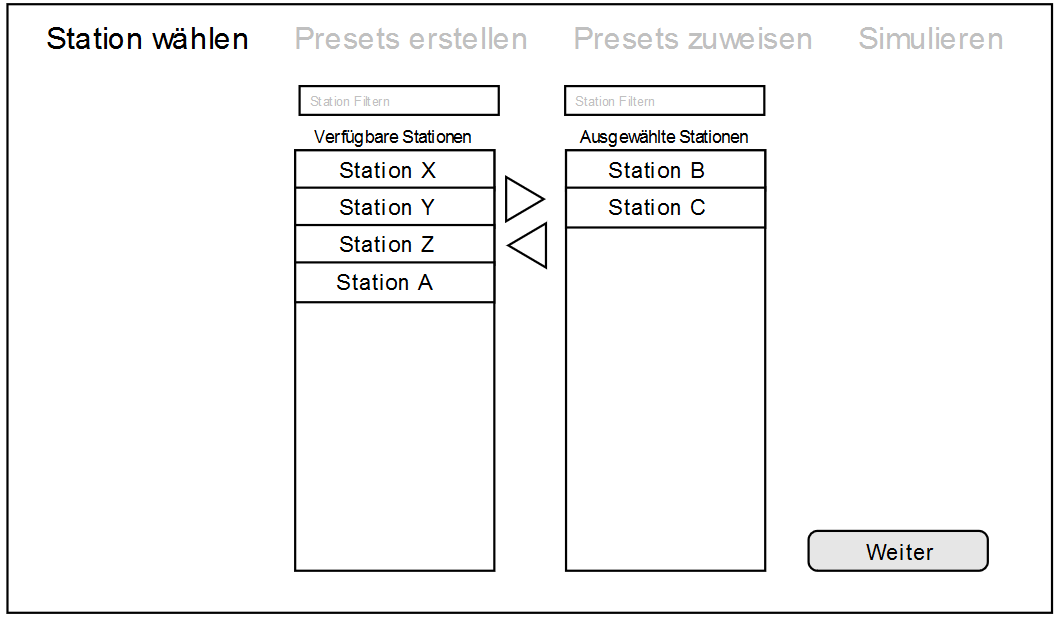
\includegraphics[width=1\textwidth]{pictures/sketches/simulator/select_sataion.png}
\caption{UI Sketch für das Auswählen von Stationen}
\label{fig:sketch_select_station}
\end{figure}
\raggedright

\subsubsection{Preset erstellen}

Um ein Preset zu erstellen muss zunächst in die korrespondierenden Felder diverse Daten eingegeben werden. Für  Minimalwert und Maximalwert bzw. Presetname wurden einfache Textfelder verwendet. Die Eingabe des Beginn- und Enddatums erfolgt durch ein Datetime Feld. Der Typ der zu generierende Messdaten, die Art der Verteilung und die Frequenz der Erstellung des Presets wird, wie in Abbildung \ref{fig:sketch_add_preset} zu sehen, mit Dropdowns festgelegt. Wenn alle Presetdaten eingegeben wurde, kann das Preset mit dem \grqq Hinzufügen\glqq-Button in die darunter befindliche Tabelle eingefügt und auch wieder entfernt werden. Nach Abschluss dieses Schittes kann wie in der Vorherigen Ansicht auf den nächsten Schritt gewechselt werden.

\begin{figure}[H]
\centering
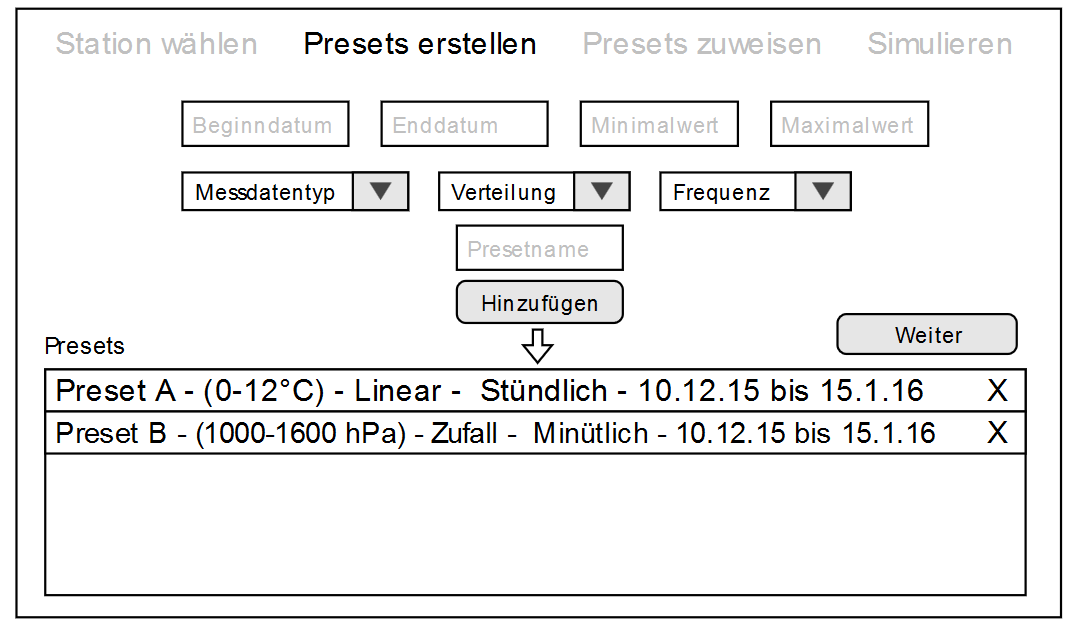
\includegraphics[width=1\textwidth]{pictures/sketches/simulator/add_presets.png}
\caption{UI Sketch für das Erstellen von Presets}
\label{fig:sketch_add_preset}
\end{figure}
\raggedright

\newpage

\subsubsection{Presets zu Stationen zuweisen}

In diesem Schritt können den einzelnen Stationen beliebig viele Presets zugewiesen werden. In Abbildung \ref{fig:sketch_assign_preset} ist zu sehen, dass per Klick auf die Station in der linken Spalte sich der Text über der mittleren Spalte ändert, damit deutlich wird, dass nun Presets zur Station B zugewiesen werden können. Das Zuweisen bzw. Löschen von Presets für die ausgewählte Station funktioniert gleich wie im ersten Schritt beschrieben. Per Klicken auf einen Eintrag der rechten Spalte, wird dieser in die mittlere Spalte verschoben und umgekehrt. Die Pfeile dienen wieder zur Verdeutlichung der gewünschten Interaktion der beiden Spalten.

\begin{figure}[H]
\centering
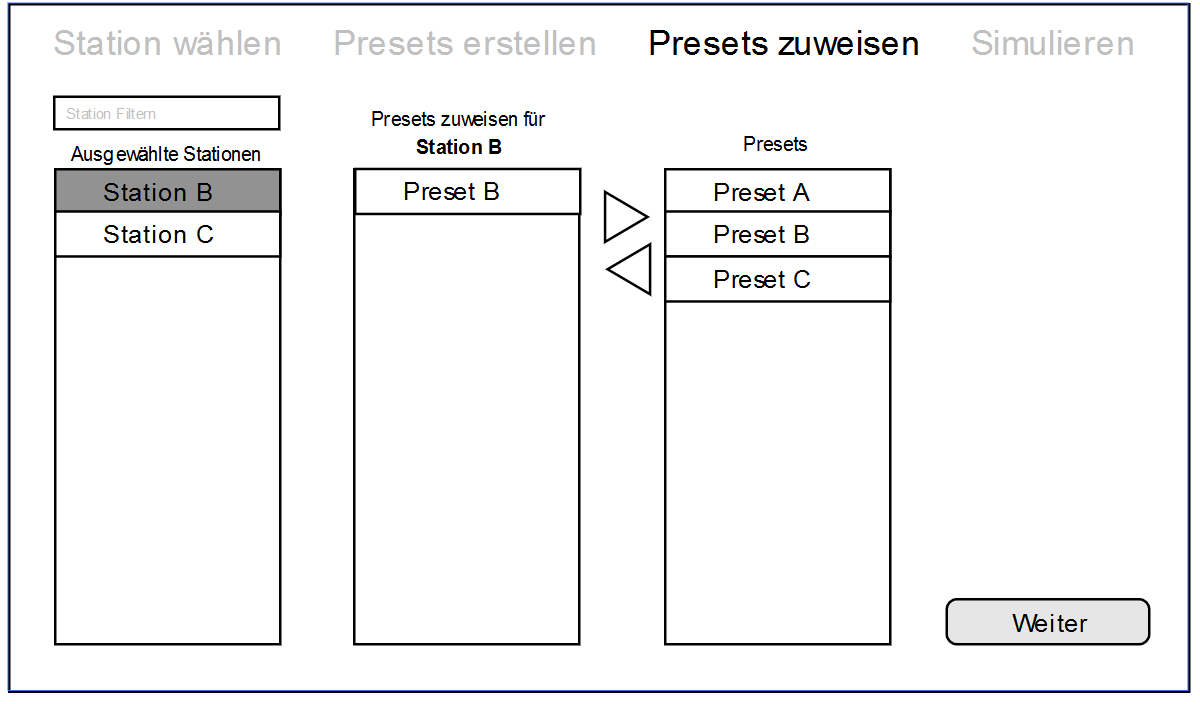
\includegraphics[width=1\textwidth]{pictures/sketches/simulator/assign_preset.png}
\caption{UI Sketch für das Zuweisen von Presets zu Stationen}
\label{fig:sketch_assign_preset}
\end{figure}
\raggedright

\newpage

\subsubsection{Simulationsübersicht}

Abbildung \ref{fig:sketch_simulation} zeigt die Liveansicht des Simulators in dem mit den zwei Buttons die Simulation gestartet oder gestoppt werden kann. Die Geschwindigkeit der Simulation, kann mit dem Slider zwischen Echtzeit und einem Vielfachen davon angepasst werden. Um bei hoher Last die Simulation zu entlasten, kann mit der Checkbox \glqq Graphen berechnen\grqq\ die Live-Visualisierung deaktiviert werden. Ansonsten wird pro in der rechten Dropdownliste ausgewählten Station für jedes zugewiesene Preset ein Graph gezeichnet, der den Verlauf der generierten Messdaten darstellt. Rechts davon befindet sich eine Liste der zugewiesenen Presets, die deaktiviert werden können, um die Visualisierung übersichtlicher zu gestellten.

\begin{figure}[H]
\centering
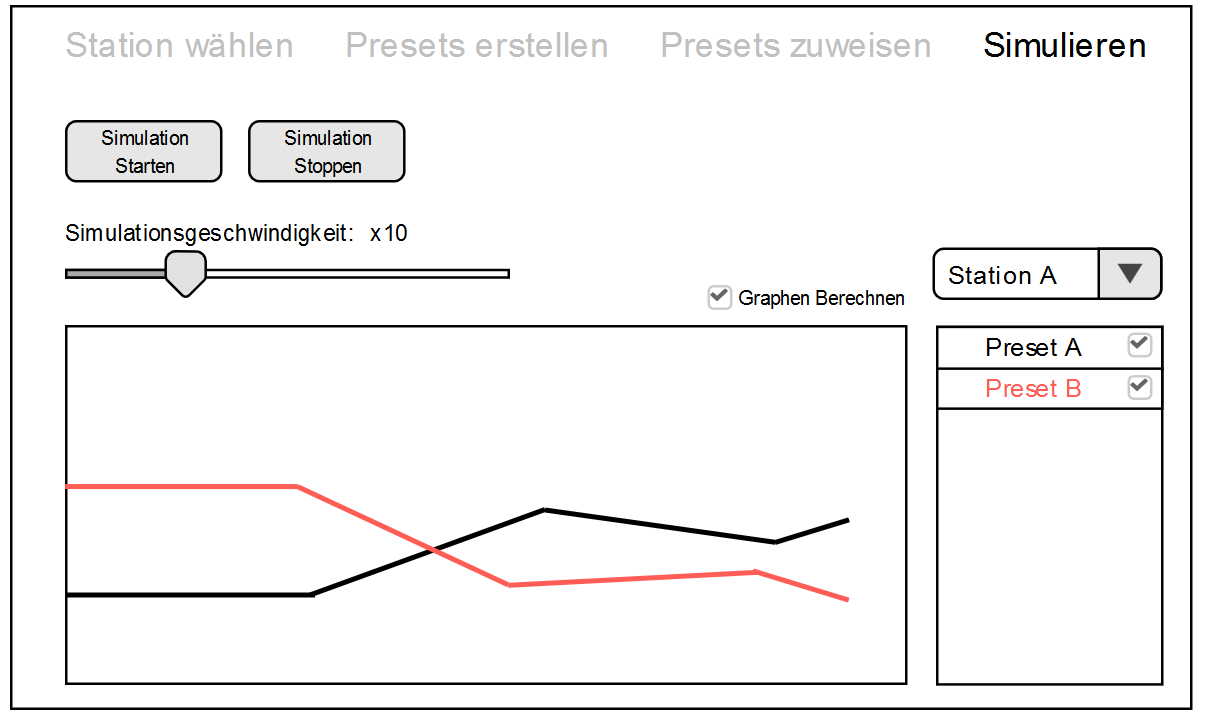
\includegraphics[width=1\textwidth]{pictures/sketches/simulator/simulate.png}
\caption{UI Sketch für die Simulationsübersicht}
\label{fig:sketch_simulation}
\end{figure}
\raggedright


\newpage

\subsection{Cockpit}

Das Cockpit besteht im wesentlichen aus drei Komponenten, welche über die linke Sidebar erreichbar sind.
\begin{itemize}
    \item Home/Dashbaord - Zeigt allgemeine Informationen und eine Wochenübericht an
    \item Analysis - Hier können komplexe Wetterabfragen getätigt werden
    \item Stationen - Verwalten der eigenen Stationen
\end{itemize}

\subsection{Login}

Die Loginmaske ist wie in Abbildung \ref{fig:cock_login} zu sehen sehr einfach gehalten. Es gibt zwei Felder, eines für die Email Adresse und eines für das Passwort. Mit dem Drücken des Login Buttons werden die eigen ebenen Daten validiert, und die anderen Bereiche freigeschaltet. Es wird automatisch auf den Homescreen bzw. das Dashboard umgeleitet.

\begin{figure}[H]
\centering
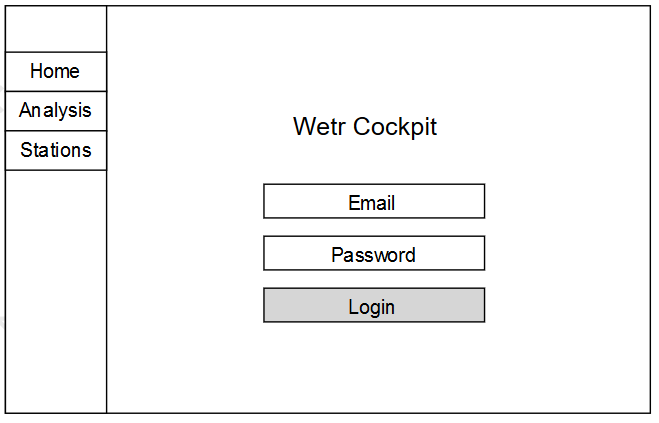
\includegraphics[width=1\textwidth]{pictures/sketches/cockpit/cockpit_login.png}
\caption{UI Sketch für die Loginmaske}
\label{fig:cock_login}
\end{figure}
\raggedright
\newpage
\subsection{Dashboard}

Hier werden allgemeine Informationen über das System (Anzahl der Stationen bzw Messdaten, u.w.) angezeigt. Die Wochenhistory (siehe Abbildung \ref{fig:cock_dash}) zeigt für die einzelnen Seiten die verschiedene Messtypen wie Temperatur oder Luftdruck an. Es kann mittels den unteren Knöpfen zwischen den Seiten gewechselt werden.

\begin{figure}[H]
\centering
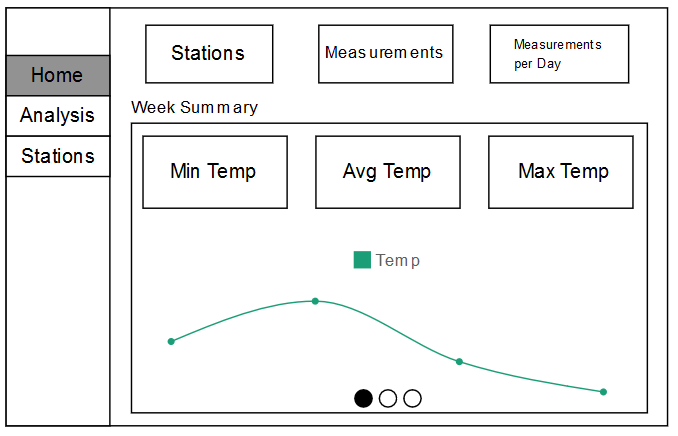
\includegraphics[width=1\textwidth]{pictures/sketches/cockpit/cockpit_home.png}
\caption{UI Sketch für das Dashboard}
\label{fig:cock_dash}
\end{figure}
\raggedright
\newpage

\subsection{Anfrage Stellen}
In dieser Ansich kann recht genau angegeben werden, welche Daten abgefragt und dargestellt werden sollen. Zu Beginn muss der Typ also Avg, Min oder Max gewählt werden. Die Gruppierung gruppiert die abgefragten Werte nach Tag, Woche oder Monat. Es muss außerdem der Messdatentyp angegeben werden. Danach kann wie in Abbildung \ref{fig:cock_query} zu sehen die Stationen gewählt werden, von denen die Daten verwendet werden solle. Wenn keine Filterung der Stationen durchgeführt wird, werden alle Stationsdaten berücksichtigt. Als letzten Schritt kann der Ort eingeschränkt werden wobei entweder Koordinaten eingegeben werden können oder anhand von bereits existierenden Orten gefiltert werden kann.

\begin{figure}[H]
\centering
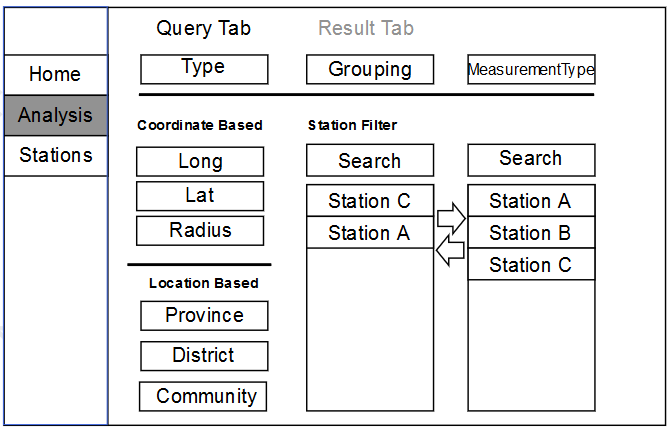
\includegraphics[width=1\textwidth]{pictures/sketches/cockpit/cockpit_query.png}
\caption{UI Sketch für das Eingeben der Abfragedaten}
\label{fig:cock_query}
\end{figure}
\raggedright
\newpage


\subsection{Ergebnis anzeigen}

Das Ergebnis der zuvor abgefragten Daten wird mittels eines Graphen (siehe Abbildung \ref{fig:cock_result}) dargestellt. Werden die Daten im Nachhinein geändert, wird der Graph neu gezeichnet.

\begin{figure}[H]
\centering
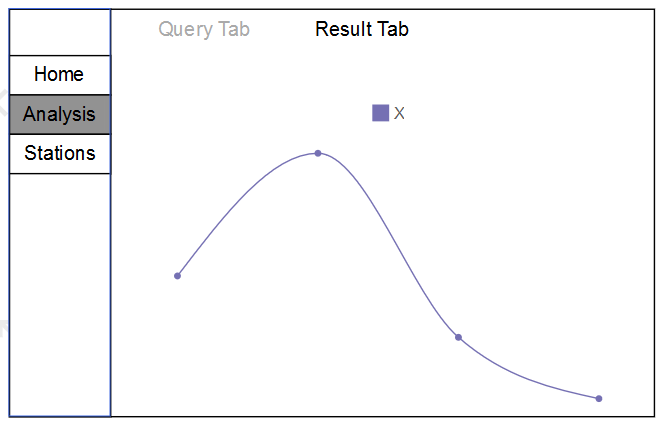
\includegraphics[width=1\textwidth]{pictures/sketches/cockpit/cockpit_result.png}
\caption{UI Sketch für Anzeigen der Resultate}
\label{fig:cock_result}
\end{figure}
\raggedright
\newpage

\subsection{Station bearbeiten}

Die in Abbildung \ref{fig:cock_edit} zeigt die Ansicht zum Editieren von den eigenen Stationen. Hierbei muss um Dropdown-Menü die zu editierende Stationen ausgewählt werden. Danach können die gezeigten Eigenschaften verändert und gespeichert werden. Das Löschen von Stationen ist nur möglich, falls noch keine Messdaten vorhanden sind.

\begin{figure}[H]
\centering
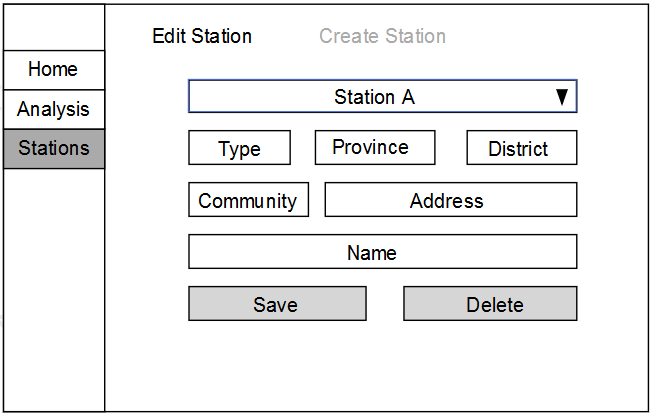
\includegraphics[width=1\textwidth]{pictures/sketches/cockpit/cockpit_edit.png}
\caption{UI Sketch für Bearbeiten der Stationen}
\label{fig:cock_edit}
\end{figure}
\raggedright
\newpage

\subsection{Station erstellen}
Das Erstellen von Stationen läuft nach dem selben Schema. Abbildung \ref{fig:cock_add} zeigt hierbei wieder das Formular mit den auszufüllenden Daten.
\begin{figure}[H]
\centering
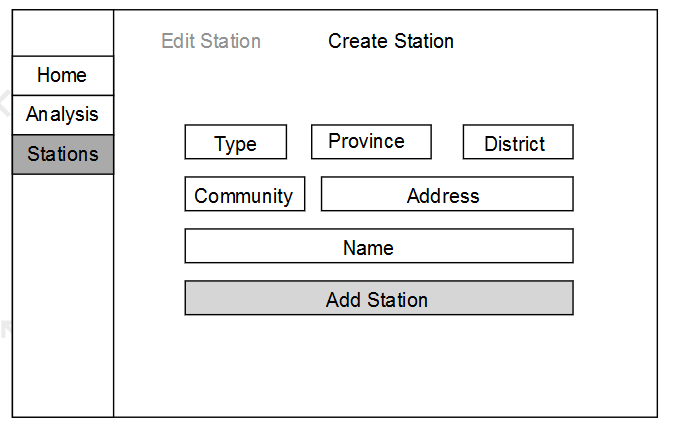
\includegraphics[width=1\textwidth]{pictures/sketches/cockpit/cockpit_create.png}
\caption{UI Sketch für Hinzufügen der Stationen}
\label{fig:cock_add}
\end{figure}
\raggedright
\newpage
